\subsection{Recurrent Neural Networks} \label{sec:background-sequence-modeling-recurrent-neural-networks}

\begin{figure}[t]
	\centering
	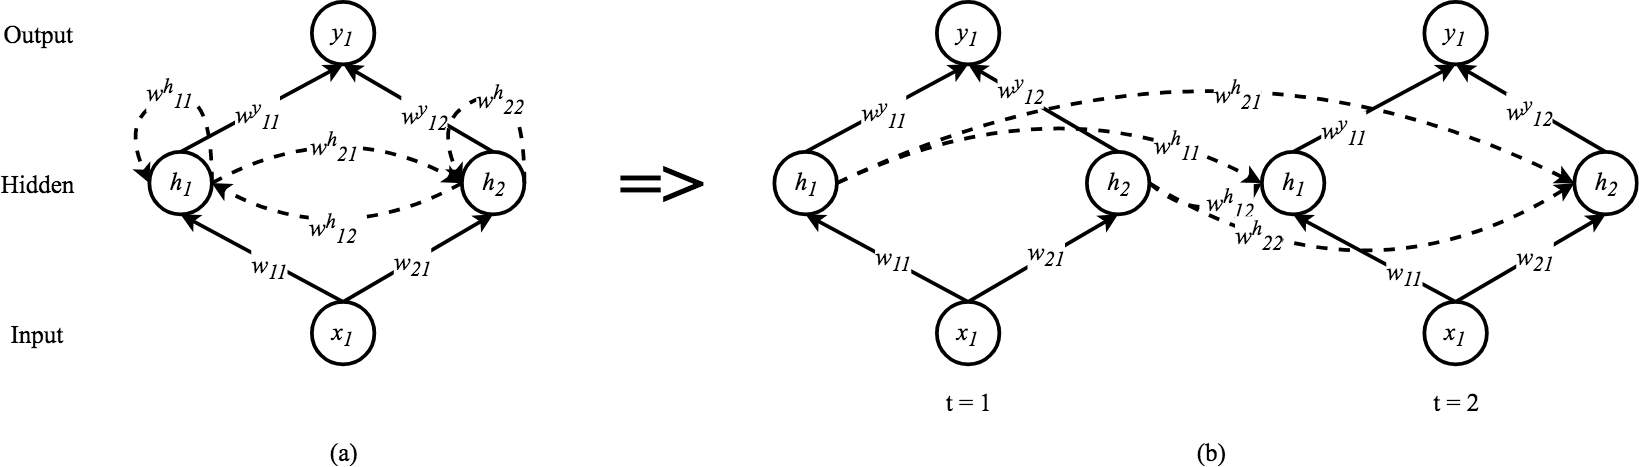
\includegraphics[max width=\textwidth]{recurrent-neural-network}
	\caption{A recurrent neural network with one hidden layer consisting of two units (a). The same neural network in (a) that is unfolded into two time steps (b)\cite{DBLP:journals/corr/Lipton15}.}
	\label{fig:recurrent-neural-network}
\end{figure}

A recurrent neural network is a feed forward neural network with additional connections between the nodes in one or more hidden layers called recurrent connections. These recurrent connections, connect the weighted output of each hidden node to another hidden node across a single time step. It is important to note that these recurrent connections do not form cycles within a single time step. The weights carried by these recurrent edges represent state that is remembered from one time step to the next and it is through this state that the recurrent neural network learns to infer context\cite{DBLP:journals/corr/Lipton15}.

Figure \ref{fig:recurrent-neural-network} (a) shows a recurrent neural network with one input unit, one output unit and a hidden layer with two units. It also shows the recurrent connections in the hidden layer. Each node in the hidden layer receives inputs from the data point $x$ and from each hidden unit $h$ in the previous time step. Figure \ref{fig:recurrent-neural-network} (b) shows the same recurrent neural network that is unfolded into two time steps. Notice that the recurrent connections are no longer depicted as cyclic connections.

Unfolding the recurrent neural network into its component time steps allows us to identify the formula used to calculate the output of each hidden node:
\begin{equation}
	h_{h}^{(t)} = \sigma(W_{hx} x^{(t)} + W_{hh} h^{(t - 1)} + b_{h})
\end{equation}
Where $W_{hx}$ is the weight matrix from the input at the current time step to the hidden unit $h$, $ x^{(t)}$ is input at the current time step, $W_{hh}$ is the weight matrix from the hidden unit $h$ at the previous time step to the same hidden unit at the current time step, $ h^{(t - 1)}$ is the output of the hidden unit $h$ from the previous time step and finally, $b_{h}$ is the bias for the hidden unit $h$\cite{DBLP:journals/corr/Lipton15}.

Unfolding recurrent neural networks also helps us visualize them as deep architectures. Each time step can be considered a layer in a deep neural network. This allows us to use the backpropagation algorithm to train recurrent neural networks using a variation known as backpropagation through time (BPTT)\cite{DBLP:journals/corr/Lipton15}.